Le Raspberry Pi est un appareil étonnant : il tient dans la poche, coûte 35 euros, et il possède pourtant toutes les caractéristiques d'un vrai ordinateur : processeur, mémoire RAM, ports USB, port jack, port HDMI, port Ethernet... Les versions les plus récentes possèdent même des puces Wi-Fi et Bluetooth directement intégrées.

\begin{figure}[h!]
\begin{center}
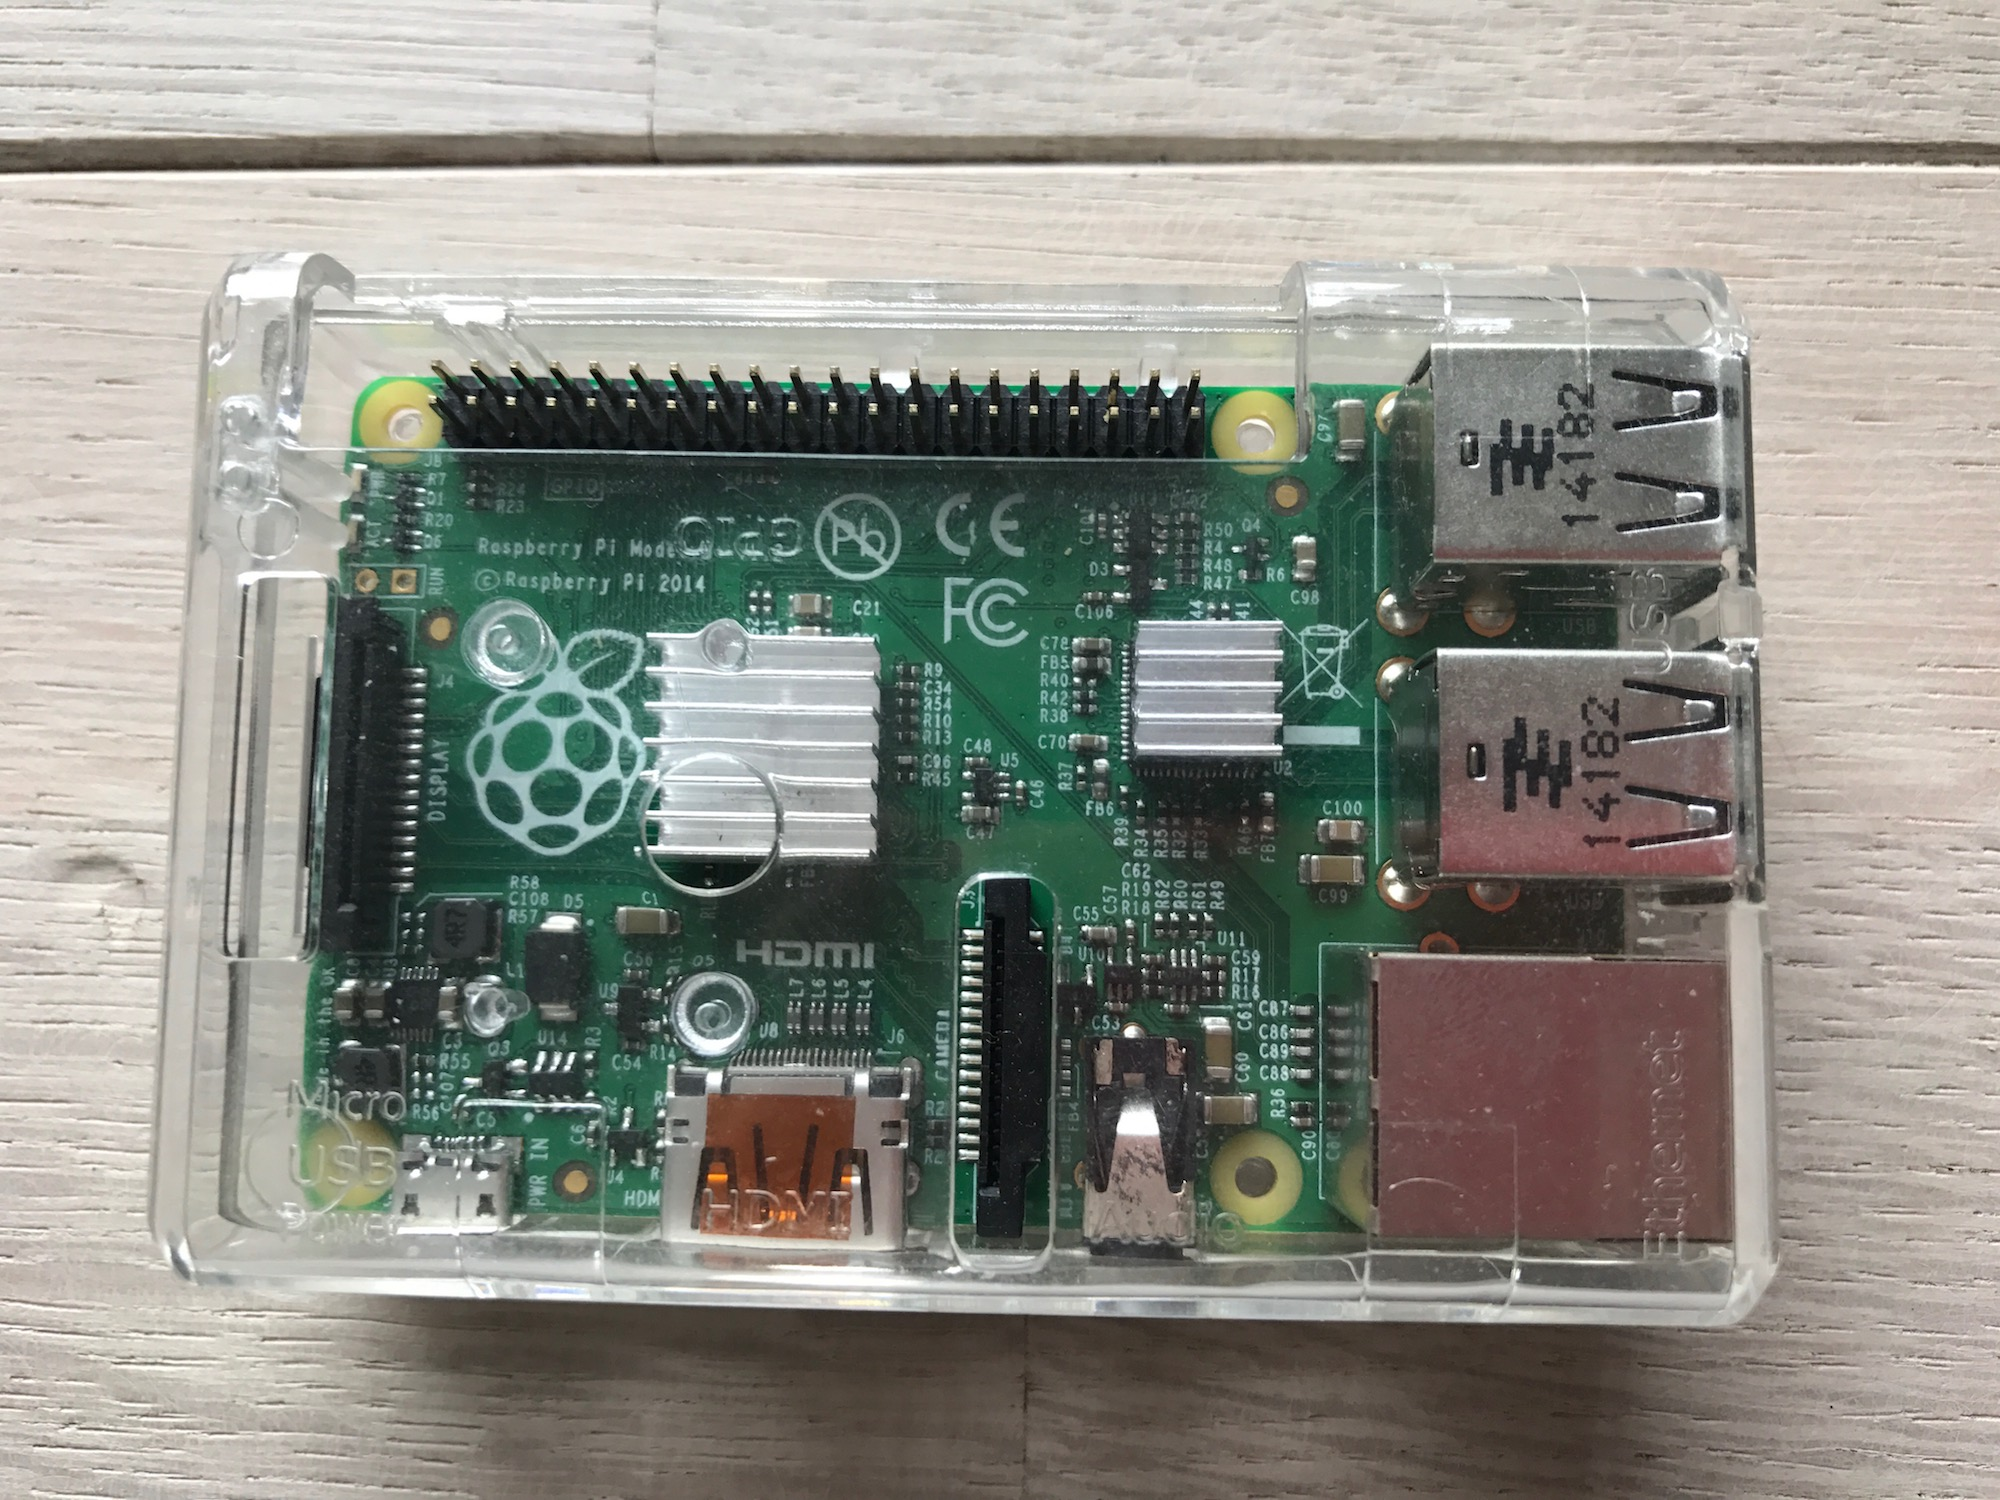
\includegraphics[width=10cm]{raspberry.JPG}
\end{center}
\caption{Raspberry Pi, première génération}
\label{raspberry}
\end{figure}

Il existe un connecteur très intéressant : les ports GPIO (\textit{General Purpose Input/Output} en anglais). Ils permettent d'envoyer ou de recevoir des signaux électriques, et de réagir en conséquence. On peut ainsi en faire de nombreux usages : allumer une LED, recevoir des informations d'un senseur, transformer une cafetière basique en une cafetière connectée... La seule limite est votre imagination!

Dans les sections suivantes, on va commencer par installer le système d'exploitation, puis on configurera l'appareil. On découvrira ensuite quelques utilisations d'un Raspberry Pi, dont certaines feront appel au Python!